\documentclass[12pt, a4paper]{article}
% --- Codificación y lenguaje ---
\usepackage[utf8]{inputenc}
\usepackage[T1]{fontenc}
\usepackage[spanish]{babel}

% --- Márgenes ---
\usepackage[top=2.5cm, bottom=2.5cm, left=3cm, right=2.5cm]{geometry}

% --- Tipografía ---
\usepackage{lmodern}

% --- Matemáticas ---
\usepackage{amsmath}
\usepackage{amssymb}

% --- Figuras y tablas ---
\usepackage{graphicx}
\usepackage{booktabs}
\usepackage{float}
\usepackage{caption}
\usepackage{subcaption}

% --- Colores ---
\usepackage{xcolor}

% --- Hipervínculos ---
\usepackage[colorlinks=true, linkcolor=blue, citecolor=blue, urlcolor=blue]{hyperref}

% --- Interlineado ---
\usepackage{setspace}
\onehalfspacing

% --- Encabezados y pies de página ---
\usepackage{fancyhdr}
\pagestyle{fancy}
\fancyhf{}
\lhead{\small Teleconexiones Climáticas}
\rhead{\small Mini Proyecto 4}
\rfoot{\thepage}

% --- Bibliografía ---
\usepackage[numbers, sort&compress]{natbib}
\bibliographystyle{plainnat}

% =============================================================
\begin{document}
	
	\begin{titlepage}
		\centering
		\vspace*{2cm}
		{\LARGE \textbf{Mini Proyecto 4: Teleconexiones Climáticas en el Eje Cafetero}\\[0.5em]
			\large Variabilidad interna del sistema climático: ENSO y la Oscilación
			Multidecadal del Atlántico como moduladores de la precipitación
			y la temperatura en los Andes colombianos}\\[2cm]
		{\large Jhon García Barrera}\\[0.5em]
		{\normalsize Física del Clima y Cambio Climático}\\[0.5em]
		{\normalsize \today}\\[3cm]
		\vfill
		{\small Código y datos disponibles en:\\
			\url{https://github.com/jhongarciab/proyectos-clima/tree/main/proyecto%204}}
	\end{titlepage}
	
	\tableofcontents
	\newpage

\section{Introducci\'on}

Colombia posee una de las mayores disponibilidades h\'idricas del planeta, y esa riqueza 
depende de manera cr\'itica del r\'egimen de precipitaci\'on sobre su vertiente Pac\'ifica 
y los Andes occidentales. Dicho r\'egimen est\'a controlado en gran medida por la 
temperatura superficial del mar (SST) en el Pac\'ifico colombiano (aproximadamente 
0--8$^{\circ}$N, 75--82$^{\circ}$W), regi\'on donde la Zona de Convergencia Intertropical 
(ITCZ) y el Chorro del Choc\'o ---la corriente de bajo nivel que transporta humedad desde 
el oc\'eano hacia el interior del pa\'is--- interact\'uan estrechamente con las condiciones 
oce\'anicas de superficie \cite{Poveda2004}. Esta conexi\'on ha sido documentada 
ampliamente: Poveda et al.\ \cite{Poveda2001} demostraron que las anomal\'ias de SST 
asociadas al fen\'omeno El Ni\~no-Oscilaci\'on del Sur (ENSO) explican hasta el 50\,\% de 
la variabilidad hidrol\'ogica colombiana, mientras que Poveda et al.\ \cite{Poveda2011} 
extendieron ese resultado mostrando la influencia adicional de la Oscilaci\'on Decadal del 
Pac\'ifico y del Atl\'antico tropical. C\'ordoba-Machado et al.\ \cite{CordobaMachado2015} 
precisaron que la precipitaci\'on en la Regi\'on Andina responde principalmente al 
Pac\'ifico central (El Ni\~no Modoki), en tanto que la Regi\'on Pac\'ifica responde al 
Pac\'ifico oriental, donde la SST local act\'ua como modulador directo de la inestabilidad 
convectiva.

A pesar de este cuerpo de evidencia, no existe una cuantificaci\'on regional de c\'omo 
responder\'ia la SST del Pac\'ifico colombiano a un forzamiento radiativo sostenido ---como 
el que impone el aumento de gases de efecto invernadero--- ni de las consecuencias 
hidrol\'ogicas de esa respuesta. Las proyecciones globales de CMIP6 \cite{Eyring2016} 
ofrecen informaci\'on sobre la SST futura a escala de cuenca, pero su resoluci\'on espacial 
es insuficiente para capturar la din\'amica local de una regi\'on tan compleja como el 
litoral Pac\'ifico colombiano, donde la orograf\'ia andina, el Chorro del Choc\'o y la 
posici\'on de la ITCZ interact\'uan a escalas de pocos grados de latitud. Esta limitaci\'on 
se agrava por el hecho de que los modelos de CMIP6 exhiben una sensibilidad clim\'atica 
m\'as alta que generaciones anteriores, en parte debido a cambios en las 
retroalimentaciones de nubes sobre el oc\'eano tropical \cite{Zelinka2020}, lo que hace 
m\'as urgente disponer de estimaciones regionales basadas en f\'isica local expl\'icita.

La capa mixta oce\'anica (CML) es la capa superficial del oc\'eano que interact\'ua 
directamente con la atm\'osfera. Su temperatura evoluciona en respuesta al balance entre 
el calentamiento solar, el enfriamiento por radiaci\'on de onda larga, los flujos 
turbulentos de calor latente y sensible, y el enfriamiento por entrainment de aguas m\'as 
fr\'ias desde abajo \cite{SwensonHansen1999}. En el Pac\'ifico tropical oriental la CML es 
delgada ---entre 15 y 50\,m seg\'un la climatolog\'ia de de Boyer Mont\'egut et al.\ 
\cite{deBoyer2004}, actualizada con perfiles Argo \cite{deBoyer2024}--- de modo que 
perturbaciones peque\~nas en el forzamiento superficial producen cambios de SST 
amplificados, haciendo a esta regi\'on especialmente sensible al calentamiento global. El 
modelo unidimensional de Price, Weller y Pinkel (PWP) \cite{Price1986} constituye una 
herramienta de referencia para simular la respuesta t\'ermica de la CML al forzamiento 
atmosf\'erico. Los flujos turbulentos en la interfaz aire-mar se parametrizan mediante el 
algoritmo COARE \cite{Fairall1996, Fairall2003}, dise\~nado espec\'ificamente para 
condiciones de viento d\'ebil y convecci\'on intensa, que son precisamente las condiciones 
prevalecientes en el Pac\'ifico colombiano.

El marco te\'orico para conectar cambios de SST con cambios de precipitaci\'on est\'a bien 
establecido. Xie et al.\ \cite{Xie2010} demostraron que bajo calentamiento global las 
lluvias aumentan donde el calentamiento local de la SST supera la media tropical y 
disminuyen donde queda por debajo; Xie \cite{Xie2020} extendi\'o ese marco mostrando que 
el patr\'on espacial de calentamiento de la SST es el principal determinante de los cambios 
regionales de precipitaci\'on en el tr\'opico. Johnson y Xie \cite{JohnsonXie2010} 
precisaron que el umbral de SST para la convecci\'on profunda se desplaza con la media 
tropical, de modo que la respuesta de precipitaci\'on a una perturbaci\'on de SST es 
predecible a primer orden. Sun et al.\ \cite{Sun2020} mostraron que el calentamiento de 
fondo de la SST amplifica la variabilidad de las lluvias en el Pac\'ifico tropical, lo que 
subraya la necesidad de resolver correctamente la respuesta t\'ermica regional. El 
debilitamiento de la circulaci\'on tropical bajo calentamiento global \cite{VecchiSoden2007} 
altera adem\'as la posici\'on de la ITCZ en funci\'on del balance energ\'etico 
interhemisf\'erico \cite{Schneider2014}, con implicaciones directas para la precipitaci\'on 
colombiana \cite{Poveda2004, Poveda2011}.

En este trabajo se implementa el modelo PWP forzado con el rean\'alisis ERA5 
\cite{Hersbach2020} para el per\'iodo 1982--2023 sobre la regi\'on 0--8$^{\circ}$N, 
75--82$^{\circ}$W. El modelo se valida contra el producto OISST v2.1 \cite{Huang2021} 
mediante RMSE, sesgo estacional y correlaci\'on de Pearson, y se verifica su capacidad 
para reproducir eventos ENSO documentados para el suroeste colombiano \cite{Ceron2021} 
y para los recursos h\'idricos del pa\'is \cite{MoralesMarın2026}. Una vez validado, el 
modelo se fuerza con perturbaciones de temperatura del aire de $+1.5^{\circ}$C, 
$+2^{\circ}$C y $+4^{\circ}$C, coherentes con los escenarios SSP1-2.6, SSP2-4.5 y 
SSP5-8.5 de CMIP6 \cite{Eyring2016}, y la respuesta t\'ermica se traduce en cambios de 
precipitaci\'on mediante una relaci\'on emp\'irica calibrada con datos CHIRPS v2 
\cite{Funk2015}. El documento se organiza as\'i: la Secci\'on~2 describe los datos y 
m\'etodos, la Secci\'on~3 presenta la validaci\'on, la Secci\'on~4 reporta los resultados 
experimentales, la Secci\'on~5 discute las limitaciones e implicaciones, y la Secci\'on~6 
sintetiza las conclusiones.

\section{Datos y m\'etodos}

\subsection{Regi\'on de estudio y conjuntos de datos}

La regi\'on de estudio comprende el Pac\'ifico colombiano entre 0--8$^{\circ}$N y 
75--82$^{\circ}$W, una franja de 957 celdas de $0.25^{\circ}$ de las cuales 541 
corresponden a superficie oce\'anica. Se emplearon cuatro conjuntos de datos (Figura~1):

\textbf{ERA5} \cite{Hersbach2020}: rean\'alisis atmosf\'erico del Centro Europeo de 
Pron\'ostico a Medio Plazo (ECMWF) con resoluci\'on horizontal de $0.25^{\circ}$ y 
frecuencia diaria. Se extrajeron temperatura del aire a 2\,m ($T_{2m}$), humedad 
espec\'ifica ($q$), velocidad del viento a 10\,m ($U_{10}$), radiaci\'on solar 
descendente en superficie (SW$\downarrow$) y radiaci\'on t\'ermica descendente en 
superficie (LW$\downarrow$), para el per\'iodo 1980--2023. La humedad espec\'ifica se 
calcul\'o a partir de la temperatura de punto de roc\'io usando la f\'ormula de Magnus, 
y la velocidad del viento como $U_{10} = \sqrt{u_{10}^2 + v_{10}^2}$.

\begin{figure}[h]
	\centering
	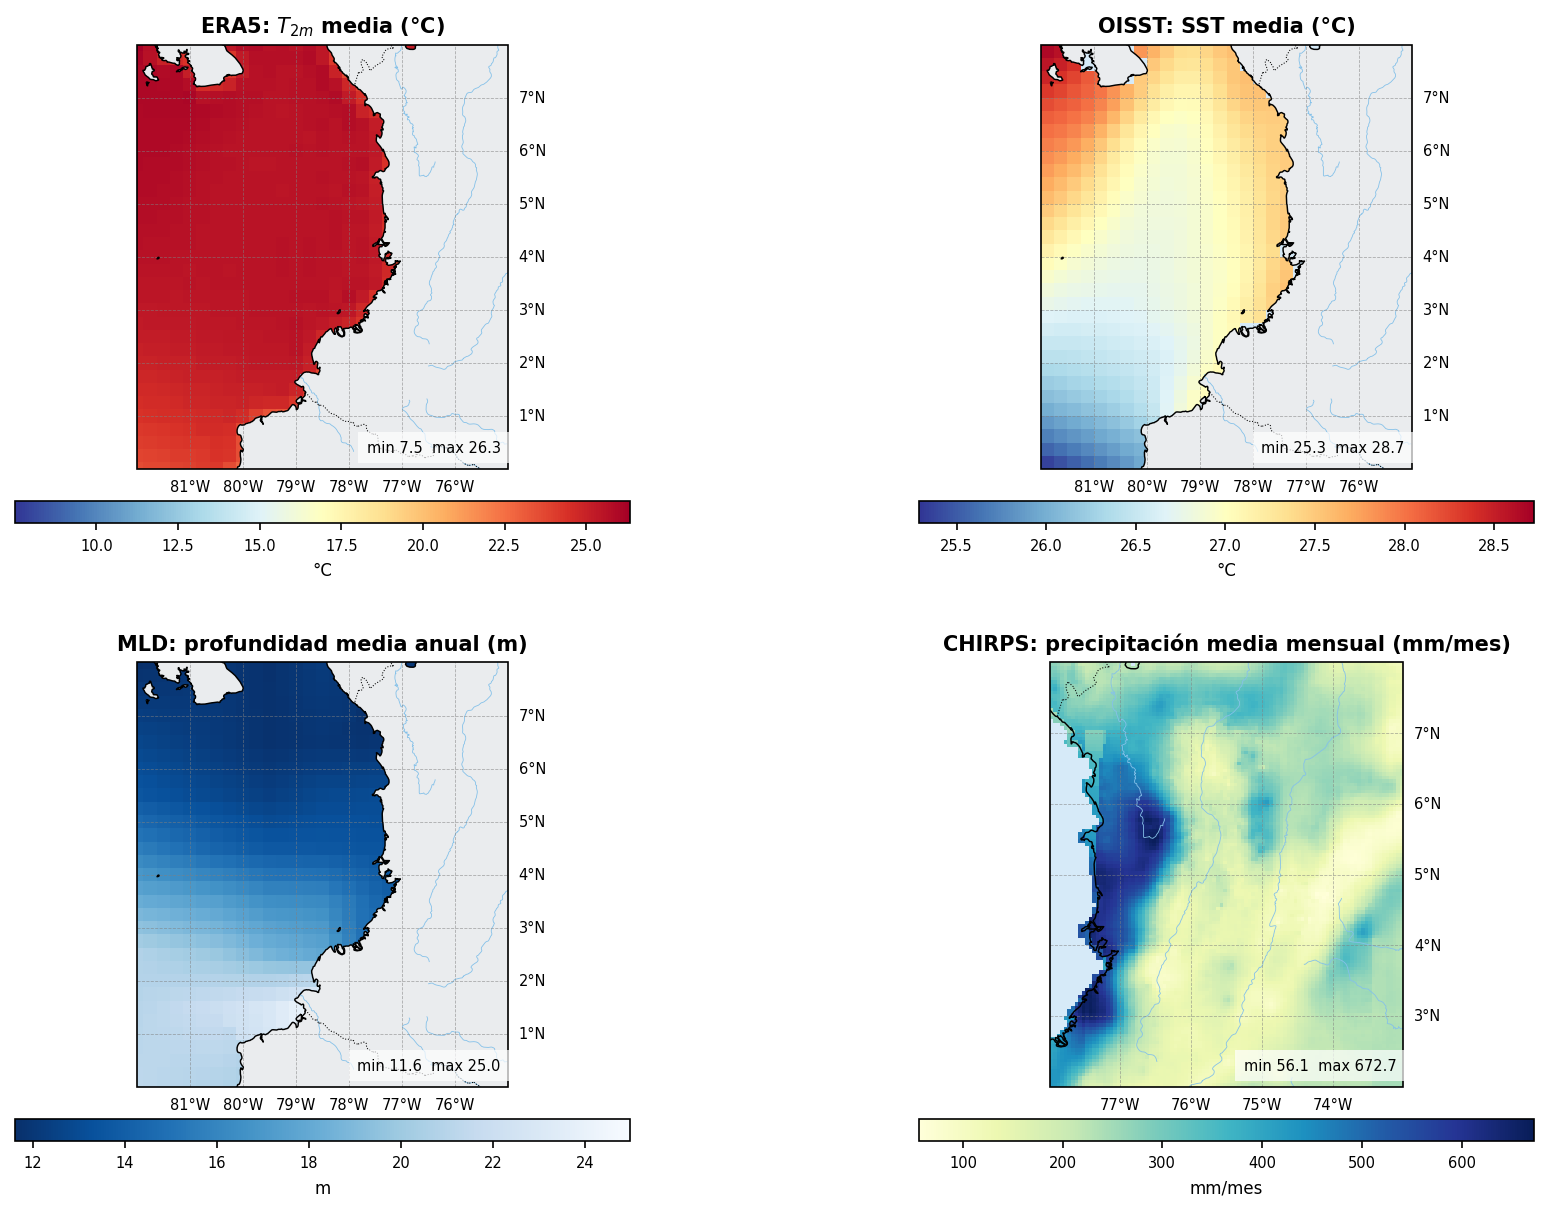
\includegraphics[width=0.80\textwidth]{../fig_control_calidad_datos.png}
	\caption{Climatolog\'ia media de los conjuntos de datos empleados sobre el 
		Pac\'ifico colombiano. (a)~Temperatura del aire a 2\,m ($T_{2m}$) de ERA5 
		(1980--2023). (b)~SST del producto OISST v2.1 (1982--2023). (c)~Profundidad 
		media anual de la capa mixta oce\'anica seg\'un la climatolog\'ia de de Boyer 
		Mont\'egut et al.\ \cite{deBoyer2004, deBoyer2024}. (d)~Precipitaci\'on media 
		mensual de CHIRPS v2 \cite{Funk2015} sobre la regi\'on costera y andina 
		adyacente (2--8$^{\circ}$N, 73--78$^{\circ}$W). Los valores m\'inimos y 
		m\'aximos de cada variable se indican en la esquina inferior derecha de cada 
		panel.}
	\label{fig:datos}
\end{figure}

\textbf{OISST v2.1} \cite{Huang2021}: producto diario de SST observada del NOAA, basado 
en sat\'elites AVHRR y boyas in situ, con resoluci\'on de $0.25^{\circ}$. Cubre el 
per\'iodo 1982--2023 (15\,340 d\'ias). Se detectaron 9 fechas faltantes, rellenas mediante 
interpolaci\'on lineal temporal; los 416 p\'ixeles de tierra presentaron valores NaN 
permanentes y fueron enmascarados. Este producto se utiliz\'o tanto como condici\'on 
inicial del modelo como referencia de validaci\'on.

\textbf{Climatolog\'ia de profundidad de la capa mixta (MLD)} 
\cite{deBoyer2004, deBoyer2024}: climatolog\'ia mensual global basada en un criterio de 
umbral de densidad de $0.03\,\text{kg\,m}^{-3}$. Para la regi\'on de estudio los valores 
oscilan entre 8.5 y 44.2\,m, con m\'inimos en el primer trimestre del a\~no. Dado que la 
climatolog\'ia original tiene resoluci\'on de $1^{\circ}$, se interpol\'o bilinealmente 
al grid ERA5 de $0.25^{\circ}$; los NaN residuales (principalmente en celdas costeras) 
se rellenaron por vecino m\'as cercano.

\textbf{CHIRPS v2} \cite{Funk2015}: precipitaci\'on mensual basada en infrarrojo y 
estaciones, con resoluci\'on de $0.05^{\circ}$. Se recort\'o la regi\'on costera y andina 
adyacente (2--8$^{\circ}$N, 73--78$^{\circ}$W, 120$\times$100 celdas) para el per\'iodo 
1981--2023, con valores mensuales entre 2.4 y 1726.3\,mm\,mes$^{-1}$.

\subsection{Modelo de capa mixta oce\'anica}

Se implement\'o el modelo unidimensional de Price, Weller y Pinkel 
\cite{Price1986} en Python. En su formulaci\'on el cambio diario de SST obedece al 
balance de calor en la CML:

\begin{equation}
	\frac{\partial T}{\partial t} = \frac{Q_\text{net}}{\rho_w c_w h} - 
	\frac{w_e \left(T - T_\text{sub}\right)}{h}
	\label{eq:pwp}
\end{equation}

\noindent donde $\rho_w = 1025\,\text{kg\,m}^{-3}$ es la densidad del agua de mar, 
$c_w = 3994\,\text{J\,kg}^{-1}\,\text{K}^{-1}$ su calor espec\'ifico, $h$ la 
profundidad de la CML tomada de la climatolog\'ia mensual, $T_\text{sub} = T - 1\,^\circ$C 
una aproximaci\'on a la temperatura subsuperficial, y $w_e$ la velocidad de entrainment 
definida como:

\begin{equation}
	w_e = \frac{\max(-Q_\text{net},\, 0)}{\rho_w c_w \left(T - T_\text{sub}\right)}
	\label{eq:we}
\end{equation}

El flujo neto de calor en superficie se calcula como:

\begin{equation}
	Q_\text{net} = (1 - \alpha)\,\text{SW}{\downarrow} + 
	\text{LW}{\downarrow} - \varepsilon\sigma T_s^4 - Q_L - Q_S
	\label{eq:qnet}
\end{equation}

\noindent con albedo $\alpha = 0.06$, emisividad $\varepsilon = 0.97$ y 
$\sigma = 5.67 \times 10^{-8}\,\text{W\,m}^{-2}\,\text{K}^{-4}$. Los flujos 
turbulentos de calor latente ($Q_L$) y sensible ($Q_S$) se calculan mediante una 
parametrizaci\'on bulk inspirada en el algoritmo COARE 
\cite{Fairall1996, Fairall2003}:

\begin{equation}
	Q_L = \rho_a L_v C_E\, U_{10}\,(q_s - q), \quad
	Q_S = \rho_a c_a C_H\, U_{10}\,(T_s - T_{2m})
	\label{eq:turb}
\end{equation}

\noindent donde $\rho_a = 1.2\,\text{kg\,m}^{-3}$, $L_v = 2.5 \times 10^6\,\text{J\,kg}^{-1}$, 
$c_a = 1005\,\text{J\,kg}^{-1}\,\text{K}^{-1}$, $C_E = 1.15 \times 10^{-3}$, 
$C_H = 1.3 \times 10^{-3}$, y $q_s$ es la humedad espec\'ifica de saturaci\'on a la 
temperatura de superficie $T_s$.

\subsection{Correci\'on del forzamiento radiativo de onda corta}

Las variables SW$\downarrow$ de ERA5 extra\'idas mediante el producto de flux medio diario 
(\texttt{avg\_sdswrf}) presentaron valores sistem\'aticamente bajos respecto a 
observaciones independientes. Una comparaci\'on con el producto CERES SYN1deg Ed4.2 para 
el per\'iodo 2001--2009 revel\'o un factor de discrepancia estable de $6.85 \pm 0.08$ 
(variaci\'on interanual), lo que apunta a un error de unidades en la cadena de 
procesamiento del producto descargado. Todas las simulaciones se realizaron con SW 
corregido por este factor, resultando en un SW$\downarrow$ medio regional de 130.1\,W\,m$^{-2}$, 
consistente con los valores reportados en la literatura para el Pac\'ifico tropical 
oriental \cite{SwensonHansen1999}. El balance energ\'etico resultante con SW corregido 
arroja un $Q_\text{net}$ medio de $+35.9\,\text{W\,m}^{-2}$ (primer a\~no de 
simulaci\'on en 4$^{\circ}$N, 80$^{\circ}$W), f\'isicamente coherente con una 
regi\'on de calentamiento neto.

\subsection{Dise\~no experimental}

El modelo se integr\'o diariamente sobre los 481 p\'ixeles oce\'anicos v\'alidos del 
dominio para el per\'iodo 1982--2023 (15\,340 d\'ias), inicializ\'andose con la SST 
observada de OISST el 1 de enero de 1982. Para los experimentos de calentamiento global 
se realizaron tres corridas adicionales id\'enticas al control pero con $T_{2m}$ 
incrementada uniformemente en $+1.5^{\circ}$C, $+2^{\circ}$C y $+4^{\circ}$C, 
coherentes con los escenarios SSP1-2.6, SSP2-4.5 y SSP5-8.5 de CMIP6 \cite{Eyring2016} 
respectivamente. Los dem\'as forzamientos (SW, LW, viento, humedad) se mantuvieron 
iguales al control, de modo que el experimento a\'isla el efecto del calentamiento 
atmosf\'erico sobre la SST.

\subsection{Relaci\'on emp\'irica SST--precipitaci\'on}

Para traducir los cambios de SST en cambios de precipitaci\'on se calibr\'o una 
regresi\'on lineal entre el \'indice regional de SST simulada (promedio espacial 
mensual sobre el dominio oce\'anico) y la precipitaci\'on media mensual de CHIRPS 
sobre la regi\'on costera y andina adyacente (2--8$^{\circ}$N, 73--78$^{\circ}$W), 
usando el per\'iodo 1982--2023 ($n = 504$ meses). Se diagnostic\'o la calidad de la 
regresi\'on mediante el coeficiente de determinaci\'on ($R^2$), el estad\'istico de 
Durbin-Watson para detectar autocorrelaci\'on en los residuales, y una regresi\'on 
adicional sobre anomal\'ias (con ciclo estacional removido) para separar la se\~nal 
interanual de la covariaci\'on estacional. La incertidumbre en la pendiente se 
cuantific\'o mediante bootstrap con 1\,000 remuestras, obteniendo un intervalo de 
confianza del 95\,\%.

\section{Validaci\'on del modelo}

\subsection{Validaci\'on temporal en el p\'ixel de referencia}

La Figura~2 muestra la serie temporal de SST simulada y observada (OISST v2.1) en el 
p\'ixel de referencia ubicado en 4$^{\circ}$N, 80$^{\circ}$W para el per\'iodo 
1982--2023. El modelo reproduce el ciclo anual y la variabilidad interanual con un RMSE 
de 1.22$^{\circ}$C, un sesgo global de $-0.11^{\circ}$C y una correlaci\'on de Pearson 
de $r = 0.659$.

\begin{figure}[h]
	\centering
	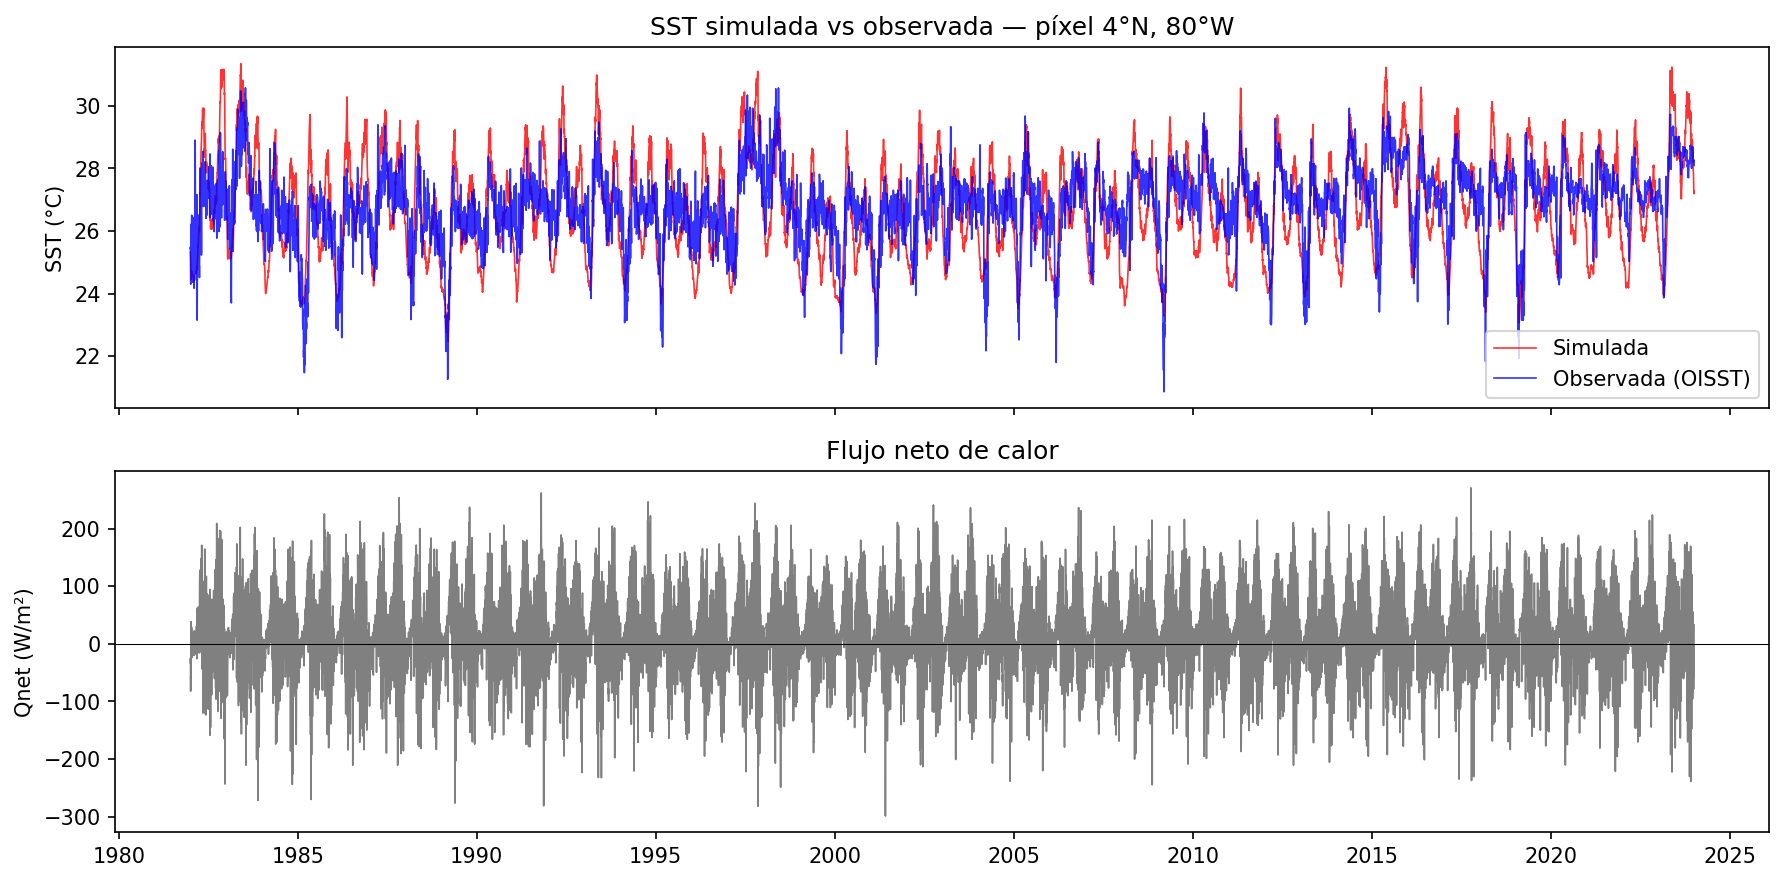
\includegraphics[width=0.80\textwidth]{../sst_simulada_vs_observada.png}
    \caption{Validaci\'on temporal del modelo PWP en el p\'ixel de referencia 
	(4$^{\circ}$N, 80$^{\circ}$W), 1982--2023. Panel superior: SST simulada (rojo) 
	y SST observada OISST v2.1 (azul). Panel inferior: flujo neto de calor en 
	superficie ($Q_\text{net}$) calculado por el modelo.}
\label{fig:validacion_temporal}
\end{figure}

\subsection{Validaci\'on espacial}

La Figura~3 presenta el mapa de diferencia entre la SST simulada media y la SST 
observada media (1982--2023) sobre el dominio oce\'anico. El RMSE espacial es de 
1.18$^{\circ}$C y el sesgo espacial de $-0.11^{\circ}$C, indicando que el modelo 
subestima ligeramente la SST en promedio. Las mayores discrepancias se concentran en 
los p\'ixeles costeros, donde la batimetr\'ia somera y los procesos de mezcla lateral 
no capturados por el modelo unidimensional introducen errores sistem\'aticos.

\begin{figure}[h]
	\centering
	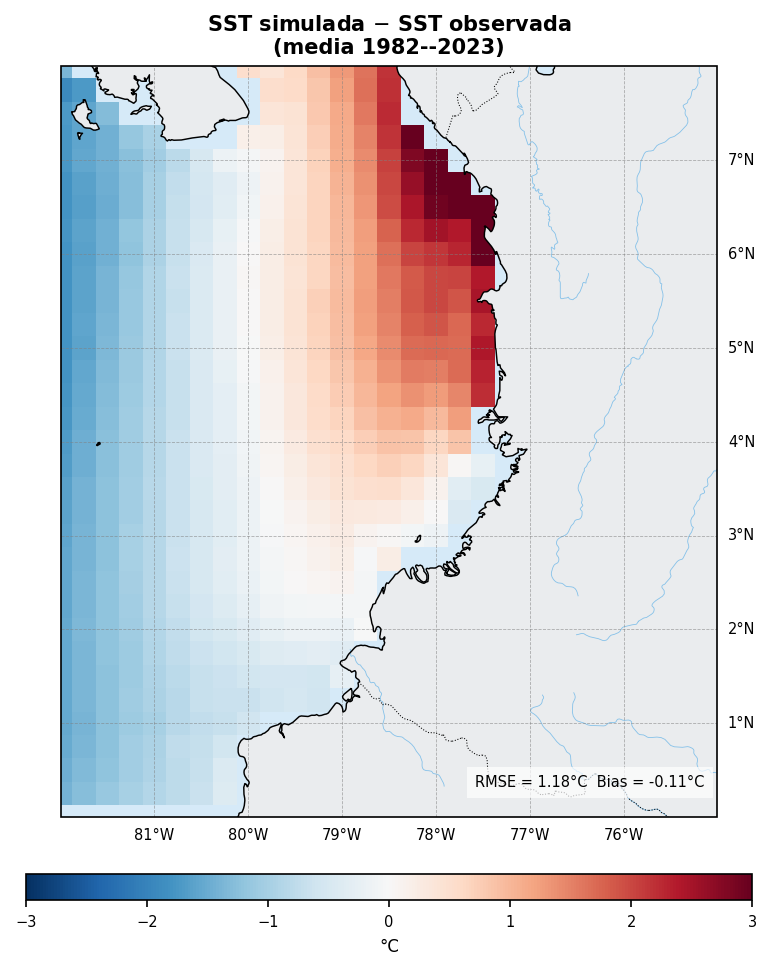
\includegraphics[width=0.45\textwidth]{../sst_simulada_vs_observada_media.png}
    \caption{Diferencia entre la SST simulada media y la SST observada media 
	(OISST v2.1) para el per\'iodo 1982--2023 sobre el dominio oce\'anico del 
	Pac\'ifico colombiano (0--8$^{\circ}$N, 75--82$^{\circ}$W). Valores positivos 
	(rojo) indican sobreestimaci\'on del modelo; valores negativos (azul) indican 
	subestimaci\'on. RMSE espacial = 1.18$^{\circ}$C, sesgo espacial = 
	$-0.11^{\circ}$C.}
\label{fig:validacion_espacial}
\end{figure}

\subsection{Validaci\'on estacional}

Las estaciones se definen por sus iniciales en ingl\'es siguiendo la convenci\'on 
meteorol\'ogica est\'andar: DJF (diciembre--febrero), MAM (marzo--mayo), JJA 
(junio--agosto) y SON (septiembre--noviembre). Las Figuras~4 y~5 descomponen 
el error por estaci\'on del a\~no. La Tabla~1 resume las m\'etricas estacionales 
espaciales sobre el dominio oce\'anico.

\begin{table}[htbp]
	\centering
	\caption{M\'etricas de validaci\'on estacional espaciales (dominio oce\'anico, 
		1982--2023).}
	\label{tab:validacion_estacional}
	\begin{tabular}{lcc}
		\hline
		Estaci\'on & RMSE ($^{\circ}$C) & Sesgo ($^{\circ}$C) \\
		\hline
		DJF & 1.70 & $-1.21$ \\
		MAM & 1.30 & $+0.22$ \\
		JJA & 1.47 & $-0.08$ \\
		SON & 1.34 & $+0.61$ \\
		\hline
		Global & 1.46 & $-0.11$ \\
		\hline
	\end{tabular}
\end{table}

DJF presenta el mayor error (RMSE = 1.70$^{\circ}$C, sesgo = $-1.21^{\circ}$C), lo que 
sugiere que el modelo subestima la SST en el primer trimestre del a\~no. Este 
comportamiento es consistente con una parametrizaci\'on de entrainment simplificada que 
tiende a enfriar en exceso la capa mixta cuando el flujo neto de calor es negativo, 
condici\'on m\'as frecuente en DJF. En contraste, JJA es la estaci\'on mejor 
reproducida en t\'erminos de sesgo ($-0.08^{\circ}$C), aunque mantiene un RMSE 
moderado de 1.47$^{\circ}$C que refleja variabilidad interanual no capturada.

\begin{figure}[htbp]
	\centering
	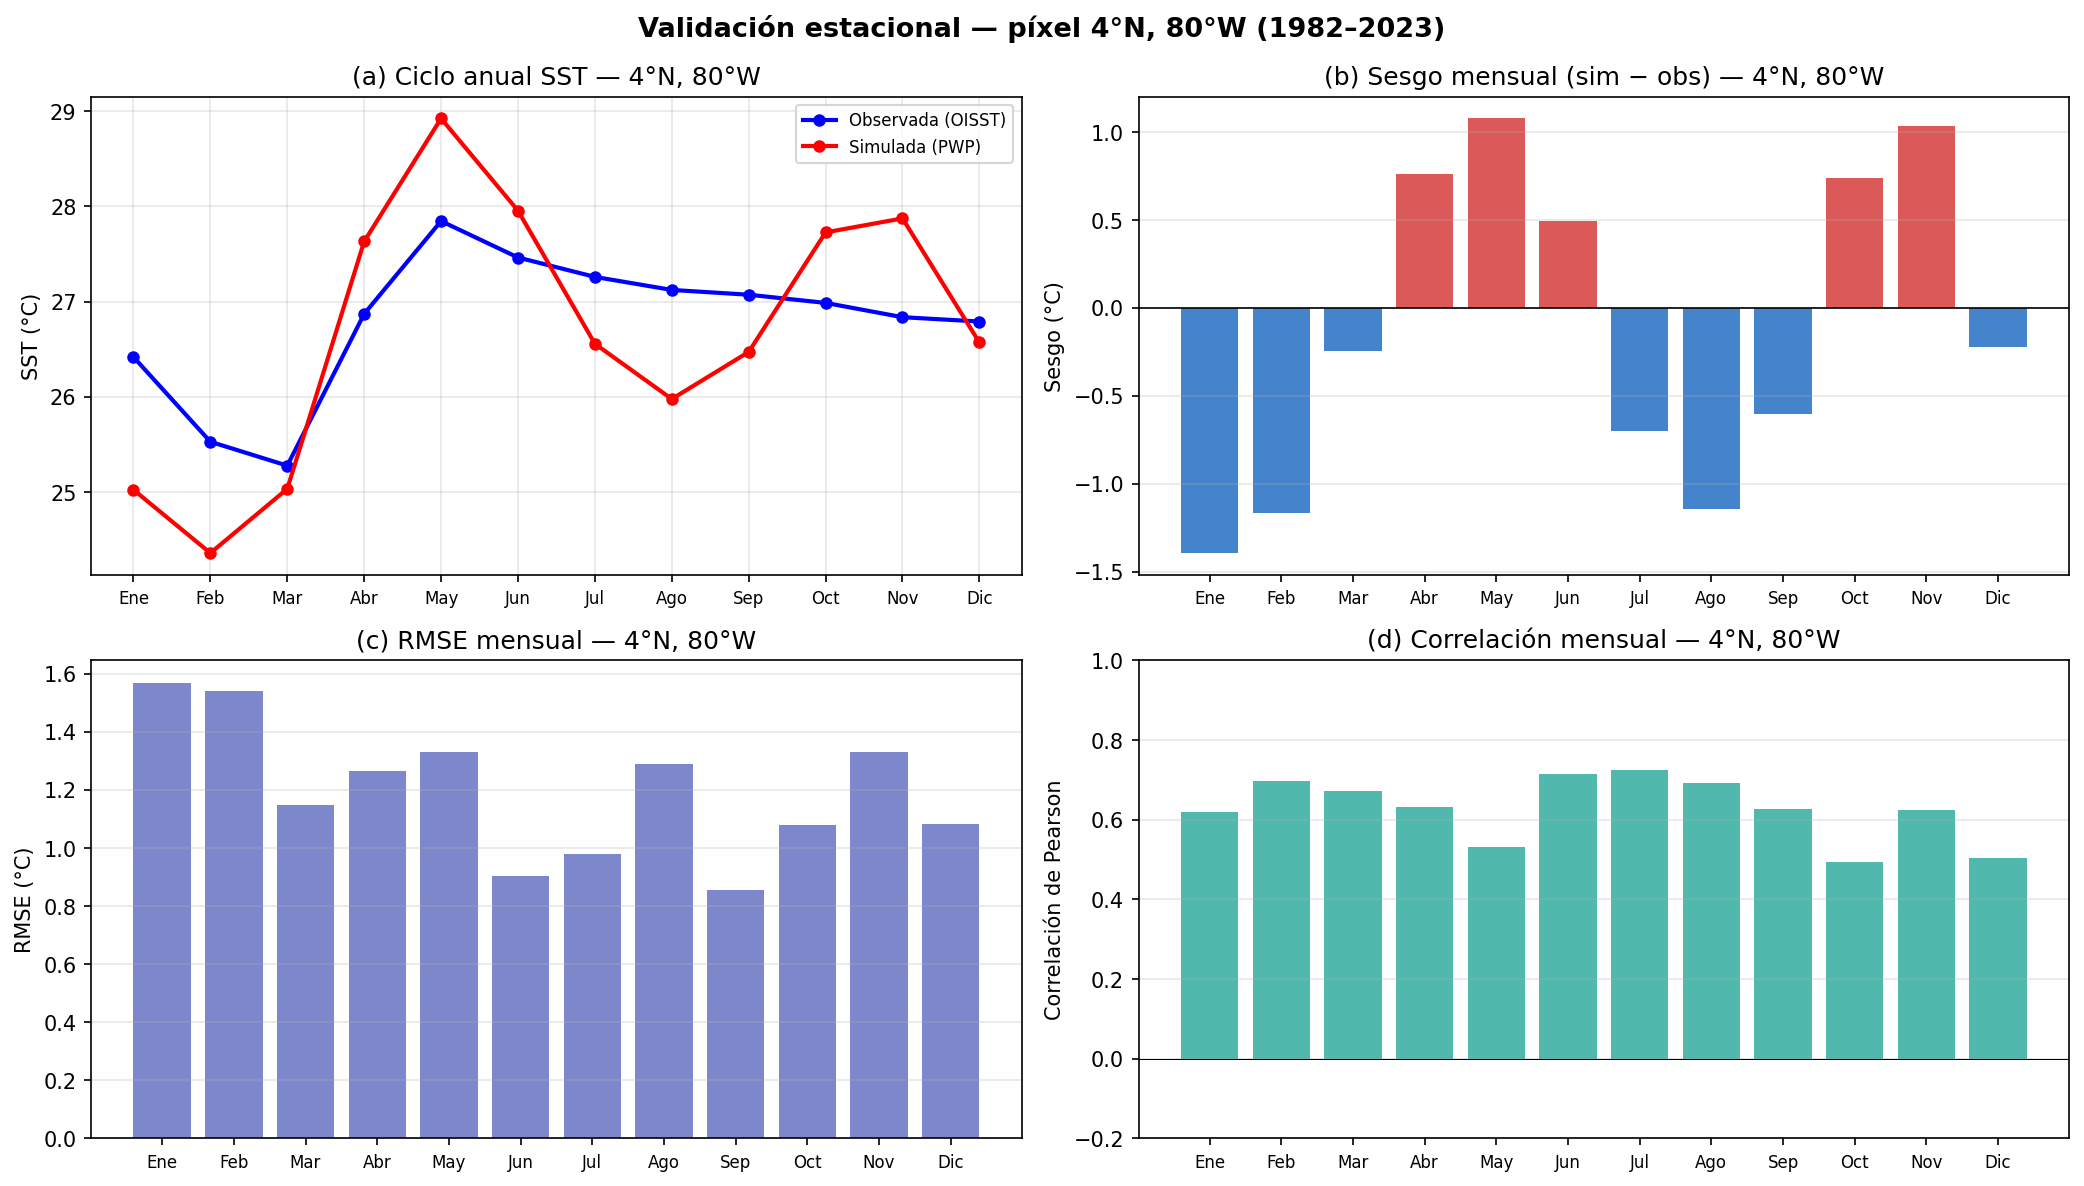
\includegraphics[width=0.65\textwidth]{../fig_validacion_estacional_pixel.png}
	\caption{Validaci\'on estacional en el p\'ixel de referencia (4$^{\circ}$N, 
		80$^{\circ}$W), 1982--2023. (a)~Ciclo anual medio de SST simulada y observada. 
		(b)~Sesgo mensual (simulada $-$ observada). (c)~RMSE mensual. 
		(d)~Correlaci\'on de Pearson mensual.}
	\label{fig:validacion_estacional_pixel}
\end{figure}

\begin{figure}[htbp]
	\centering
	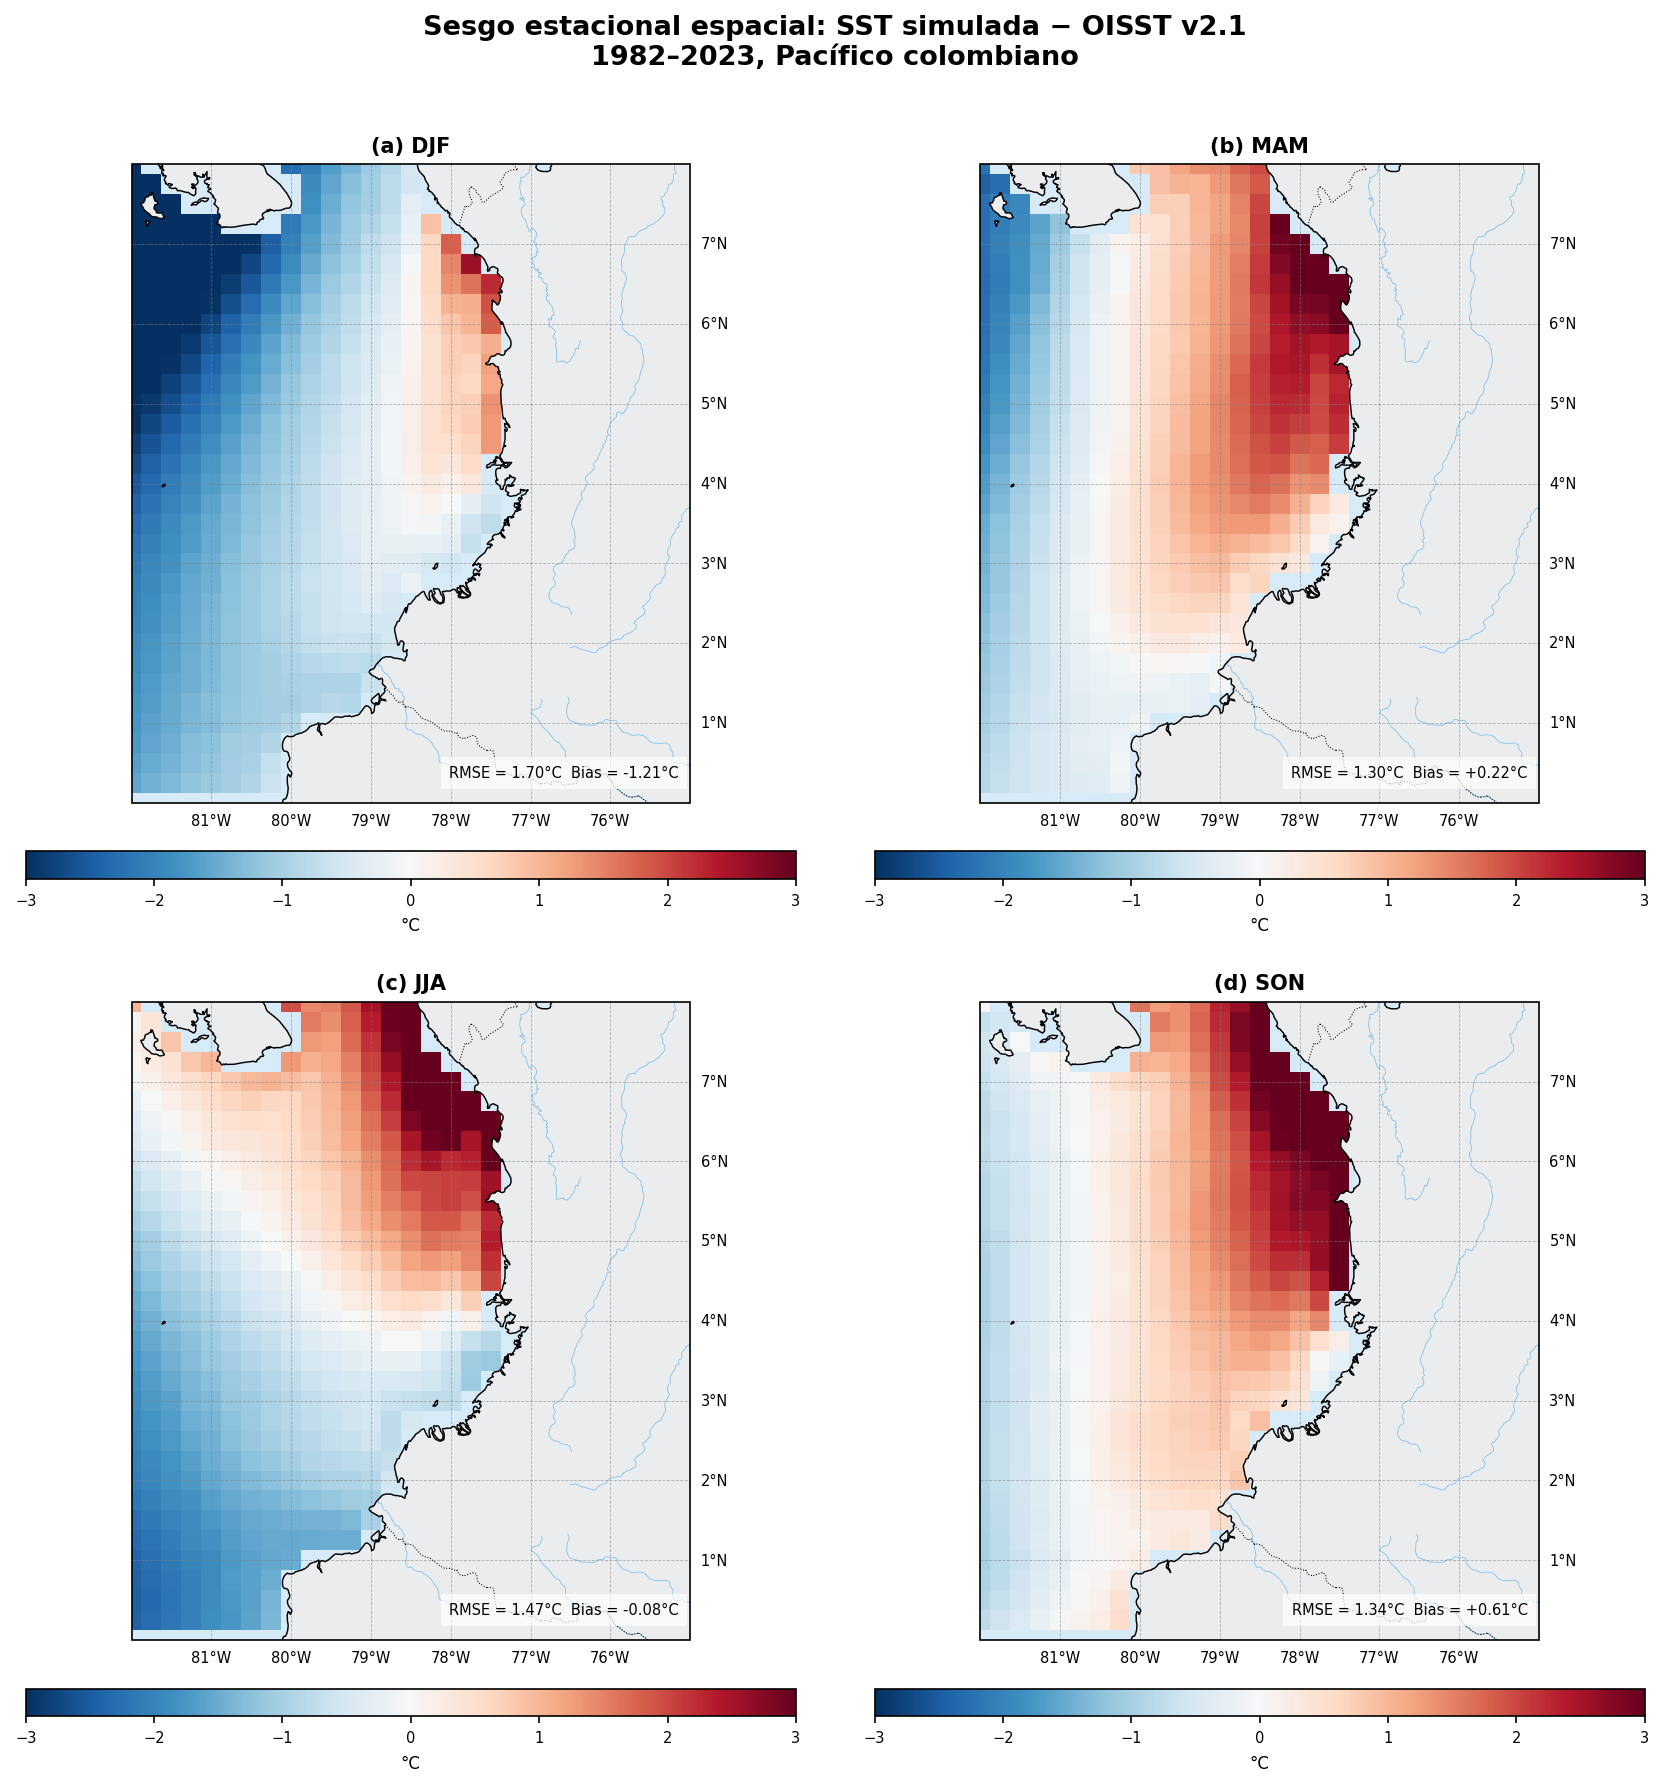
\includegraphics[width=0.65\textwidth]{../fig_validacion_estacional_mapas.png}
	\caption{Sesgo espacial estacional (SST simulada $-$ OISST v2.1, media 
		1982--2023) sobre el dominio oce\'anico del Pac\'ifico colombiano. 
		(a)~DJF (diciembre--febrero). (b)~MAM (marzo--mayo). (c)~JJA 
		(junio--agosto). (d)~SON (septiembre--noviembre). Las m\'etricas RMSE y 
		sesgo medio de cada estaci\'on se indican en la esquina inferior derecha 
		de cada panel.}
	\label{fig:validacion_estacional_mapas}
\end{figure}

\subsection{Reproducci\'on de eventos ENSO}

La Figura~6 muestra las anomal\'ias de SST simulada y observada en 4$^{\circ}$N, 
80$^{\circ}$W con los principales eventos ENSO sombreados. La Tabla~2 cuantifica la 
anomal\'ia media durante cada evento.

\begin{table}[htbp]
	\centering
	\caption{Anomal\'ia media de SST simulada y observada durante eventos ENSO 
		documentados (p\'ixel 4$^{\circ}$N, 80$^{\circ}$W).}
	\label{tab:enso}
	\begin{tabular}{lccc}
		\hline
		Evento & Obs ($^{\circ}$C) & Sim ($^{\circ}$C) & Signo correcto \\
		\hline
		El Ni\~no 1982--83 & $+0.63$ & $+1.35$ & \checkmark \\
		La Ni\~na 1988--89 & $-0.99$ & $-0.97$ & \checkmark \\
		El Ni\~no 1997--98 & $+1.58$ & $+1.60$ & \checkmark \\
		La Ni\~na 1999--00 & $-0.71$ & $-0.97$ & \checkmark \\
		La Ni\~na 2010--11 & $+0.28$ & $-0.39$ & $\times$ \\
		El Ni\~no 2015--16 & $+0.99$ & $+1.21$ & \checkmark \\
		\hline
	\end{tabular}
\end{table}

El modelo reproduce correctamente el signo de la anomal\'ia en 5 de los 6 eventos 
considerados. La excepci\'on es La Ni\~na 2010--11, donde la observaci\'on registra 
una anomal\'ia ligeramente positiva ($+0.28^{\circ}$C) que el modelo simula como 
negativa ($-0.39^{\circ}$C); la magnitud observada es peque\~na y puede estar 
influenciada por factores locales no representados en el modelo. Para los eventos de 
mayor se\~nal (El Ni\~no 1997--98 y La Ni\~na 1988--89), la correspondencia entre 
simulaci\'on y observaci\'on es muy estrecha, lo que indica que el modelo captura 
adecuadamente la respuesta t\'ermica de la capa mixta a las anomal\'ias de forzamiento 
asociadas a ENSO.

\begin{figure}[htbp]
	\centering
	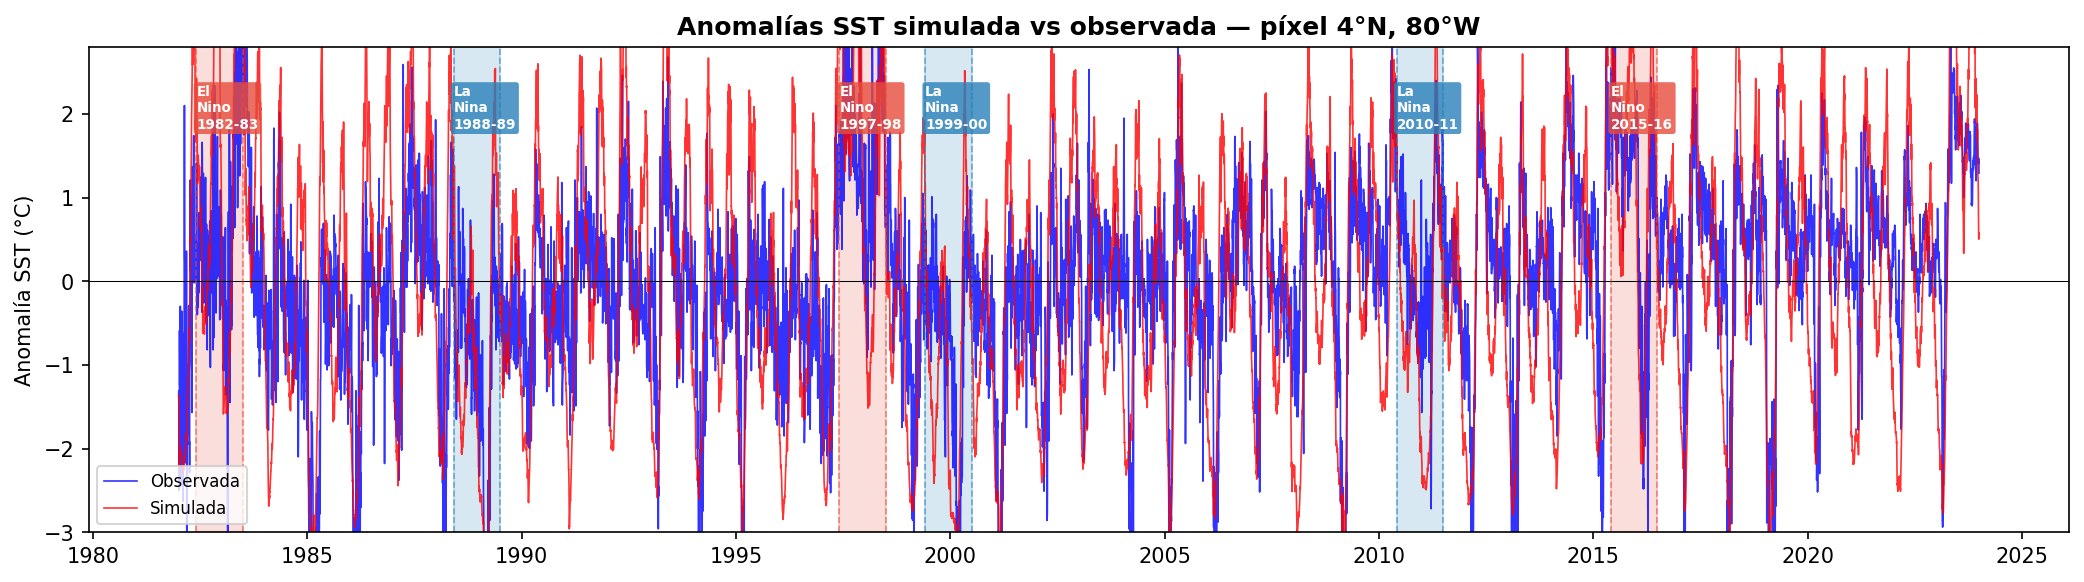
\includegraphics[width=\textwidth]{../fig_anomalias_enso.png}
	\caption{Anomal\'ias de SST simulada (rojo) y observada (azul, OISST v2.1) 
		en el p\'ixel de referencia (4$^{\circ}$N, 80$^{\circ}$W) para el per\'iodo 
		1982--2023. Las regiones sombreadas indican eventos El Ni\~no (rojo) y 
		La Ni\~na (azul) documentados para el Pac\'ifico colombiano 
		\cite{Ceron2021, MoralesMarın2026}. Las anomal\'ias se calcularon respecto 
		a la media climatol\'ogica del per\'iodo completo.}
	\label{fig:anomalias_enso}
\end{figure}

\section{Resultados}

\subsection{Respuesta t\'ermica de la SST por escenario}

\begin{figure}[h]
	\centering
	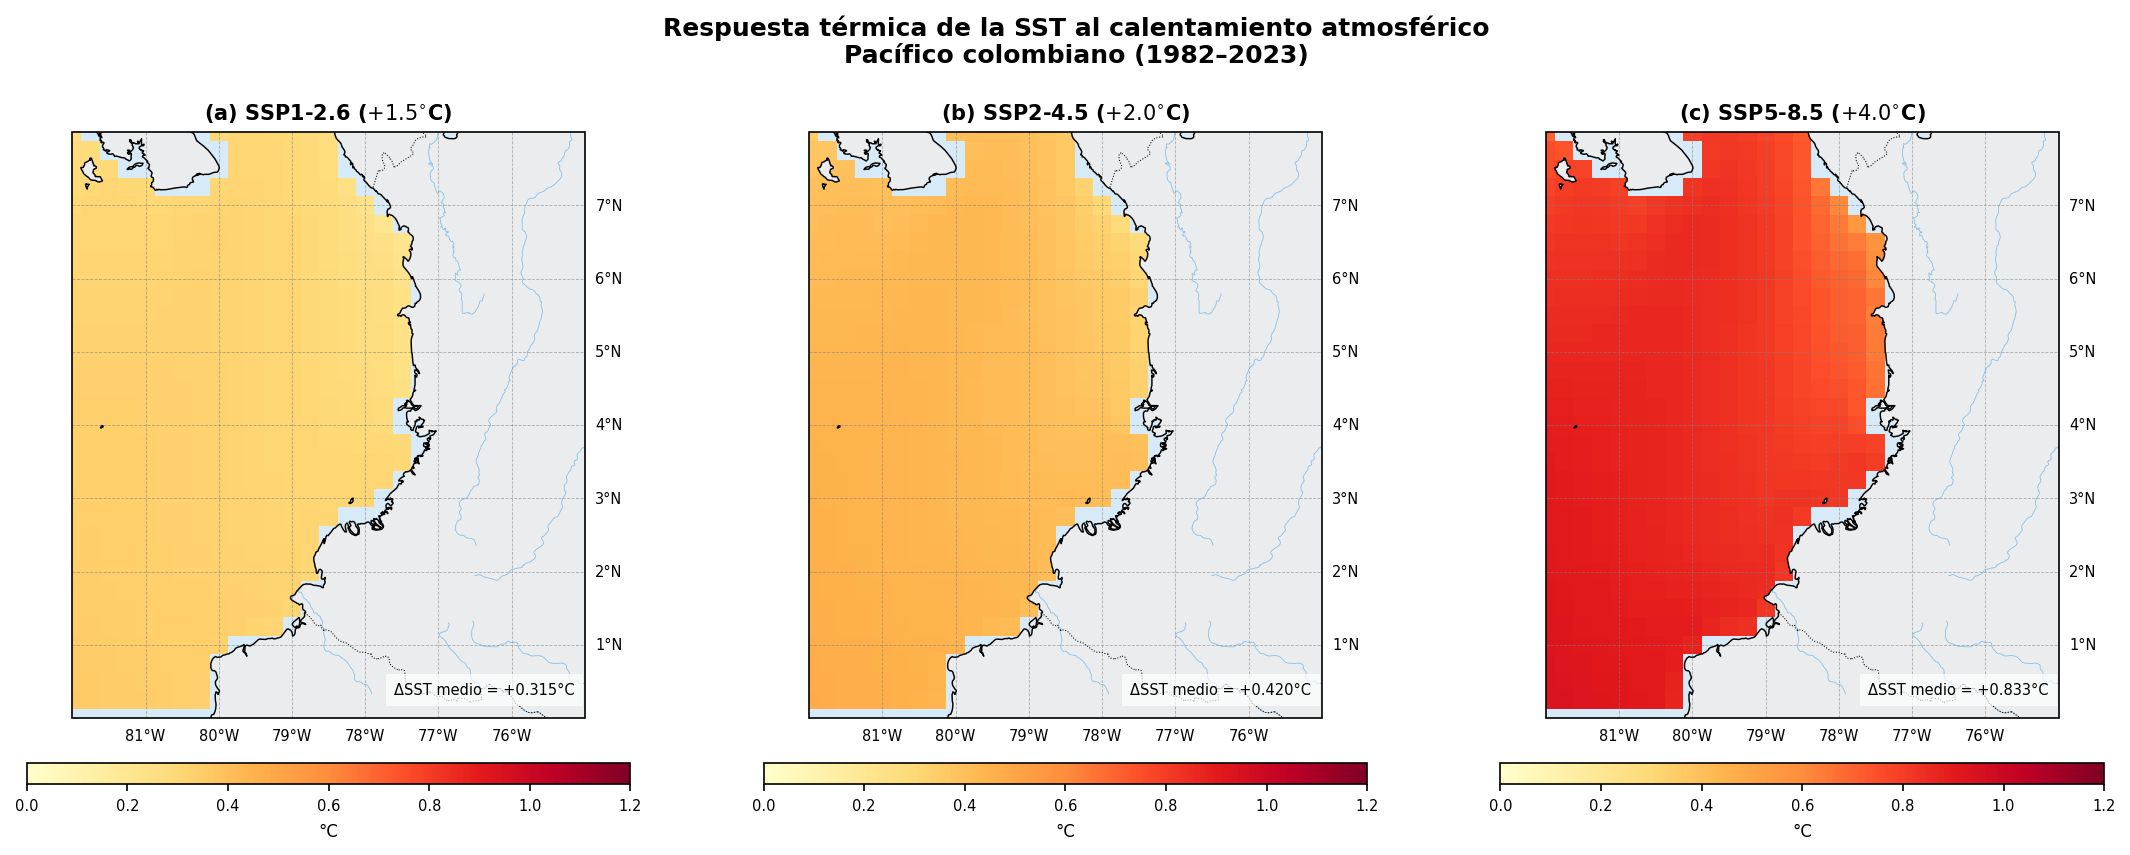
\includegraphics[width=\textwidth]{../fig_delta_sst_escenarios.png}
	\caption{Cambio medio en SST ($\Delta$SST, promedio 1982--2023) respecto al control 
		para los tres escenarios de calentamiento atmosf\'erico. (a)~SSP1-2.6 
		($+1.5^{\circ}$C), $\Delta$SST medio = $+0.32^{\circ}$C. (b)~SSP2-4.5 
		($+2.0^{\circ}$C), $\Delta$SST medio = $+0.42^{\circ}$C. (c)~SSP5-8.5 
		($+4.0^{\circ}$C), $\Delta$SST medio = $+0.83^{\circ}$C. En los tres casos el 
		calentamiento de la SST es inferior a la perturbaci\'on impuesta en $T_{2m}$, 
		reflejando el efecto amortiguador de los flujos turbulentos y el entrainment.}
	\label{fig:delta_sst_escenarios}
\end{figure}

La Figura~7 presenta los mapas de $\Delta$SST medio (diferencia entre cada experimento 
y el control, promediada sobre 1982--2023) para los tres escenarios.
El calentamiento medio del dominio es de $+0.32^{\circ}$C para SSP1-2.6, 
$+0.42^{\circ}$C para SSP2-4.5 y $+0.83^{\circ}$C para SSP5-8.5. En los tres casos 
el $\Delta$SST es inferior a la perturbaci\'on impuesta en $T_{2m}$ ($+1.5^{\circ}$C, 
$+2^{\circ}$C y $+4^{\circ}$C respectivamente), lo que refleja el efecto amortiguador 
del entrainment y de los flujos turbulentos: al aumentar $T_{2m}$, el gradiente 
aire-mar se reduce, disminuye el calor sensible cedido al oc\'eano y aumenta la 
evaporaci\'on, limitando el calentamiento neto de la CML. La respuesta no es 
espacialmente uniforme --- los p\'ixeles del sector norte del dominio (6--8$^{\circ}$N) 
muestran $\Delta$SST sistem\'aticamente mayores, consistente con una CML m\'as delgada 
en esa subregi\'on seg\'un la climatolog\'ia de MLD.

Por otro lado, la Figura~8 muestra el ciclo anual del $\Delta$SST promediado sobre el dominio 
oce\'anico.

\begin{figure}[h]
	\centering
	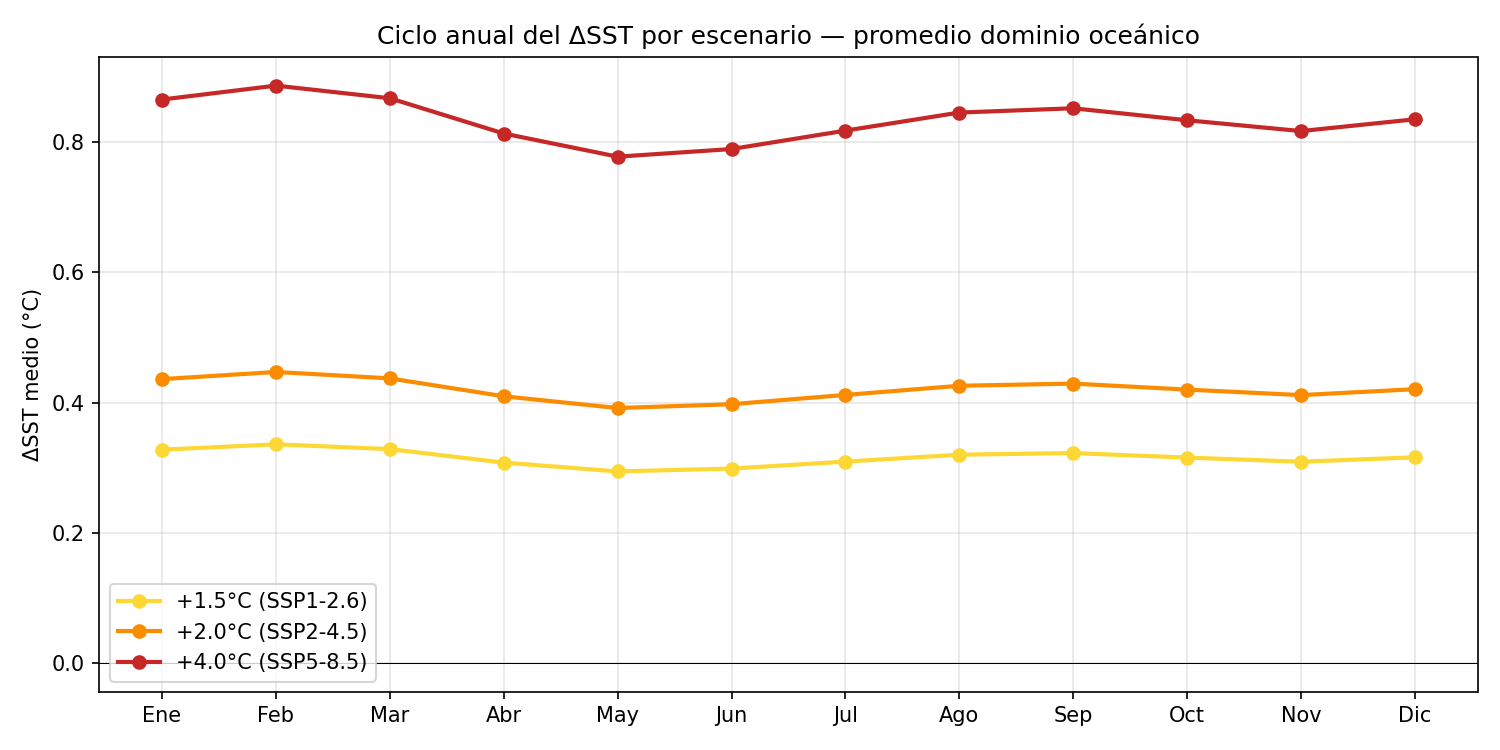
\includegraphics[width=0.80\textwidth]{../fig_ciclo_anual_delta_sst.png}
	\caption{Ciclo anual del $\Delta$SST medio sobre el dominio oce\'anico del 
		Pac\'ifico colombiano para los tres escenarios de calentamiento. Los mayores 
		calentamientos ocurren entre junio y octubre, coincidiendo con el per\'iodo 
		de menor profundidad de la CML.}
	\label{fig:ciclo_anual_delta_sst}
\end{figure}

El ciclo anual revela una dependencia estacional moderada: los mayores calentamientos 
ocurren entre junio y octubre, coincidiendo con el per\'iodo de menor profundidad de 
la CML, cuando una misma anomal\'ia de $Q_\text{net}$ produce cambios de temperatura 
m\'as amplios seg\'un la ecuaci\'on~(\ref{eq:pwp}).

\subsection{Mecanismo: balance de calor bajo calentamiento}

La Figura~9 descompone el cambio en cada componente del balance de calor entre el 
escenario SSP5-8.5 ($+4^{\circ}$C) y el control, promediado sobre el dominio oce\'anico. 
Los resultados muestran que el aumento de $T_{2m}$ produce:

\begin{itemize}
	\item $\Delta Q_S = -21.9\,\text{W\,m}^{-2}$: reducci\'on del calor sensible cedido 
	al oc\'eano, porque el gradiente $T_s - T_{2m}$ se reduce al calentarse el aire.
	\item $\Delta Q_L = +17.2\,\text{W\,m}^{-2}$: aumento del calor latente (mayor 
	evaporaci\'on), porque la SST tambi\'en sube ligeramente y aumenta $q_s$.
	\item $\Delta Q_{LW} = -5.0\,\text{W\,m}^{-2}$: mayor p\'erdida de onda larga 
	emitida por el oc\'eano al aumentar $T_s$.
	\item $\Delta Q_{SW} = 0.0\,\text{W\,m}^{-2}$: sin cambio, porque SW$\downarrow$ 
	no se perturba en el experimento.
\end{itemize}

\begin{figure}[htbp]
	\centering
	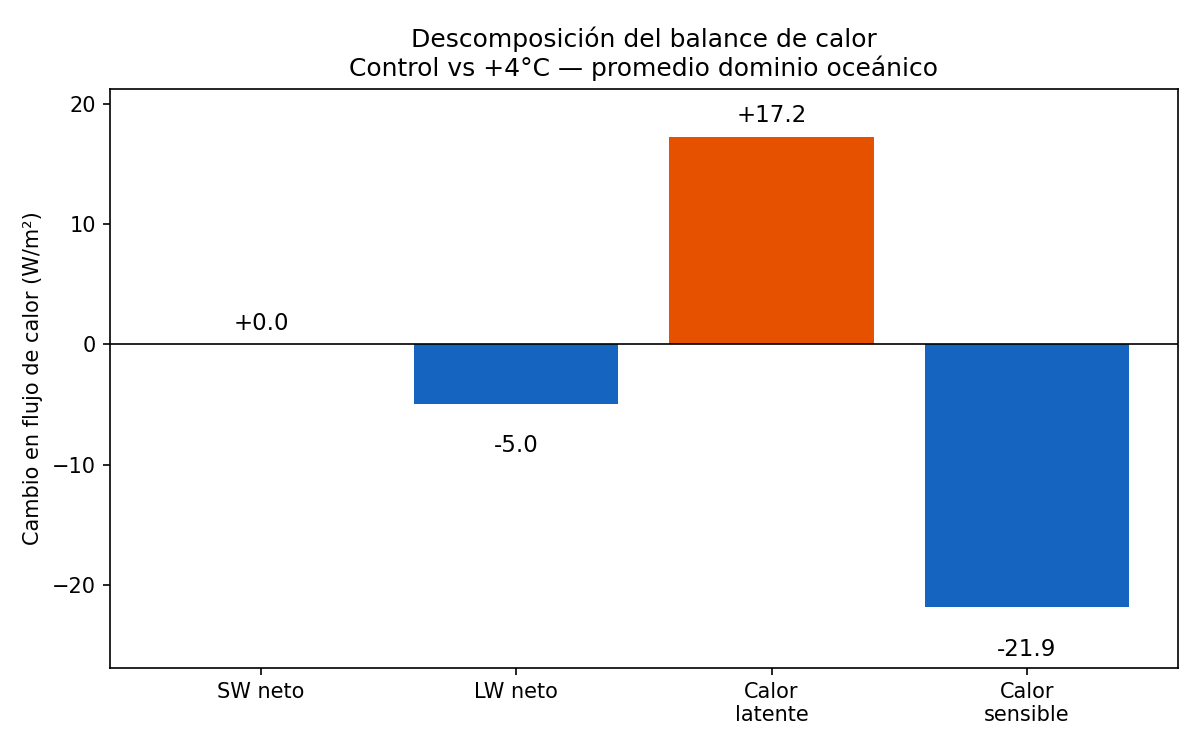
\includegraphics[width=0.75\textwidth]{../fig_balance_calor.png}
	\caption{Cambio en las componentes del balance de calor superficial entre el 
		escenario SSP5-8.5 ($+4^{\circ}$C) y el control, promediado sobre el dominio 
		oce\'anico del Pac\'ifico colombiano (1982--2023). Barras naranja: incremento 
		neto de calor hacia el oc\'eano; barras azul: reducci\'on neta. El balance 
		resultante ($\Delta Q_\text{net} \approx -0.4\,\text{W\,m}^{-2}$) es 
		pr\'acticamente nulo, lo que explica la convergencia del $\Delta$SST a un 
		nuevo equilibrio.}
	\label{fig:balance_calor}
\end{figure}

El balance neto es $\Delta Q_\text{net} \approx -0.4\,\text{W\,m}^{-2}$, pr\'acticamente 
nulo, lo que explica por qu\'e el $\Delta$SST converge a un nuevo equilibrio en lugar de 
derivar indefinidamente. El mecanismo dominante es la compensaci\'on entre la 
reducci\'on del calor sensible (que tender\'ia a calentar la CML) y el aumento de la 
evaporaci\'on (que la enfr\'ia): el resultado neto es un calentamiento modesto pero 
persistente de la SST.

\subsection{Relaci\'on SST--precipitaci\'on y estimaci\'on de cambios}

La Figura~10 presenta el diagn\'ostico completo de la calibraci\'on SST--precipitaci\'on 
para el per\'iodo 1982--2023 ($n = 504$ meses). La regresi\'on sobre series brutas 
arroja una pendiente de $31.7\,\text{mm\,mes}^{-1}\,^{\circ}\text{C}^{-1}$ 
($R^2 = 0.364$, $p < 10^{-50}$, $\text{SE} = 1.9\,\text{mm\,mes}^{-1}\,^{\circ}\text{C}^{-1}$), 
lo que sugiere una relaci\'on positiva aparentemente robusta entre SST y precipitaci\'on. 

\begin{figure}[h]
	\centering
	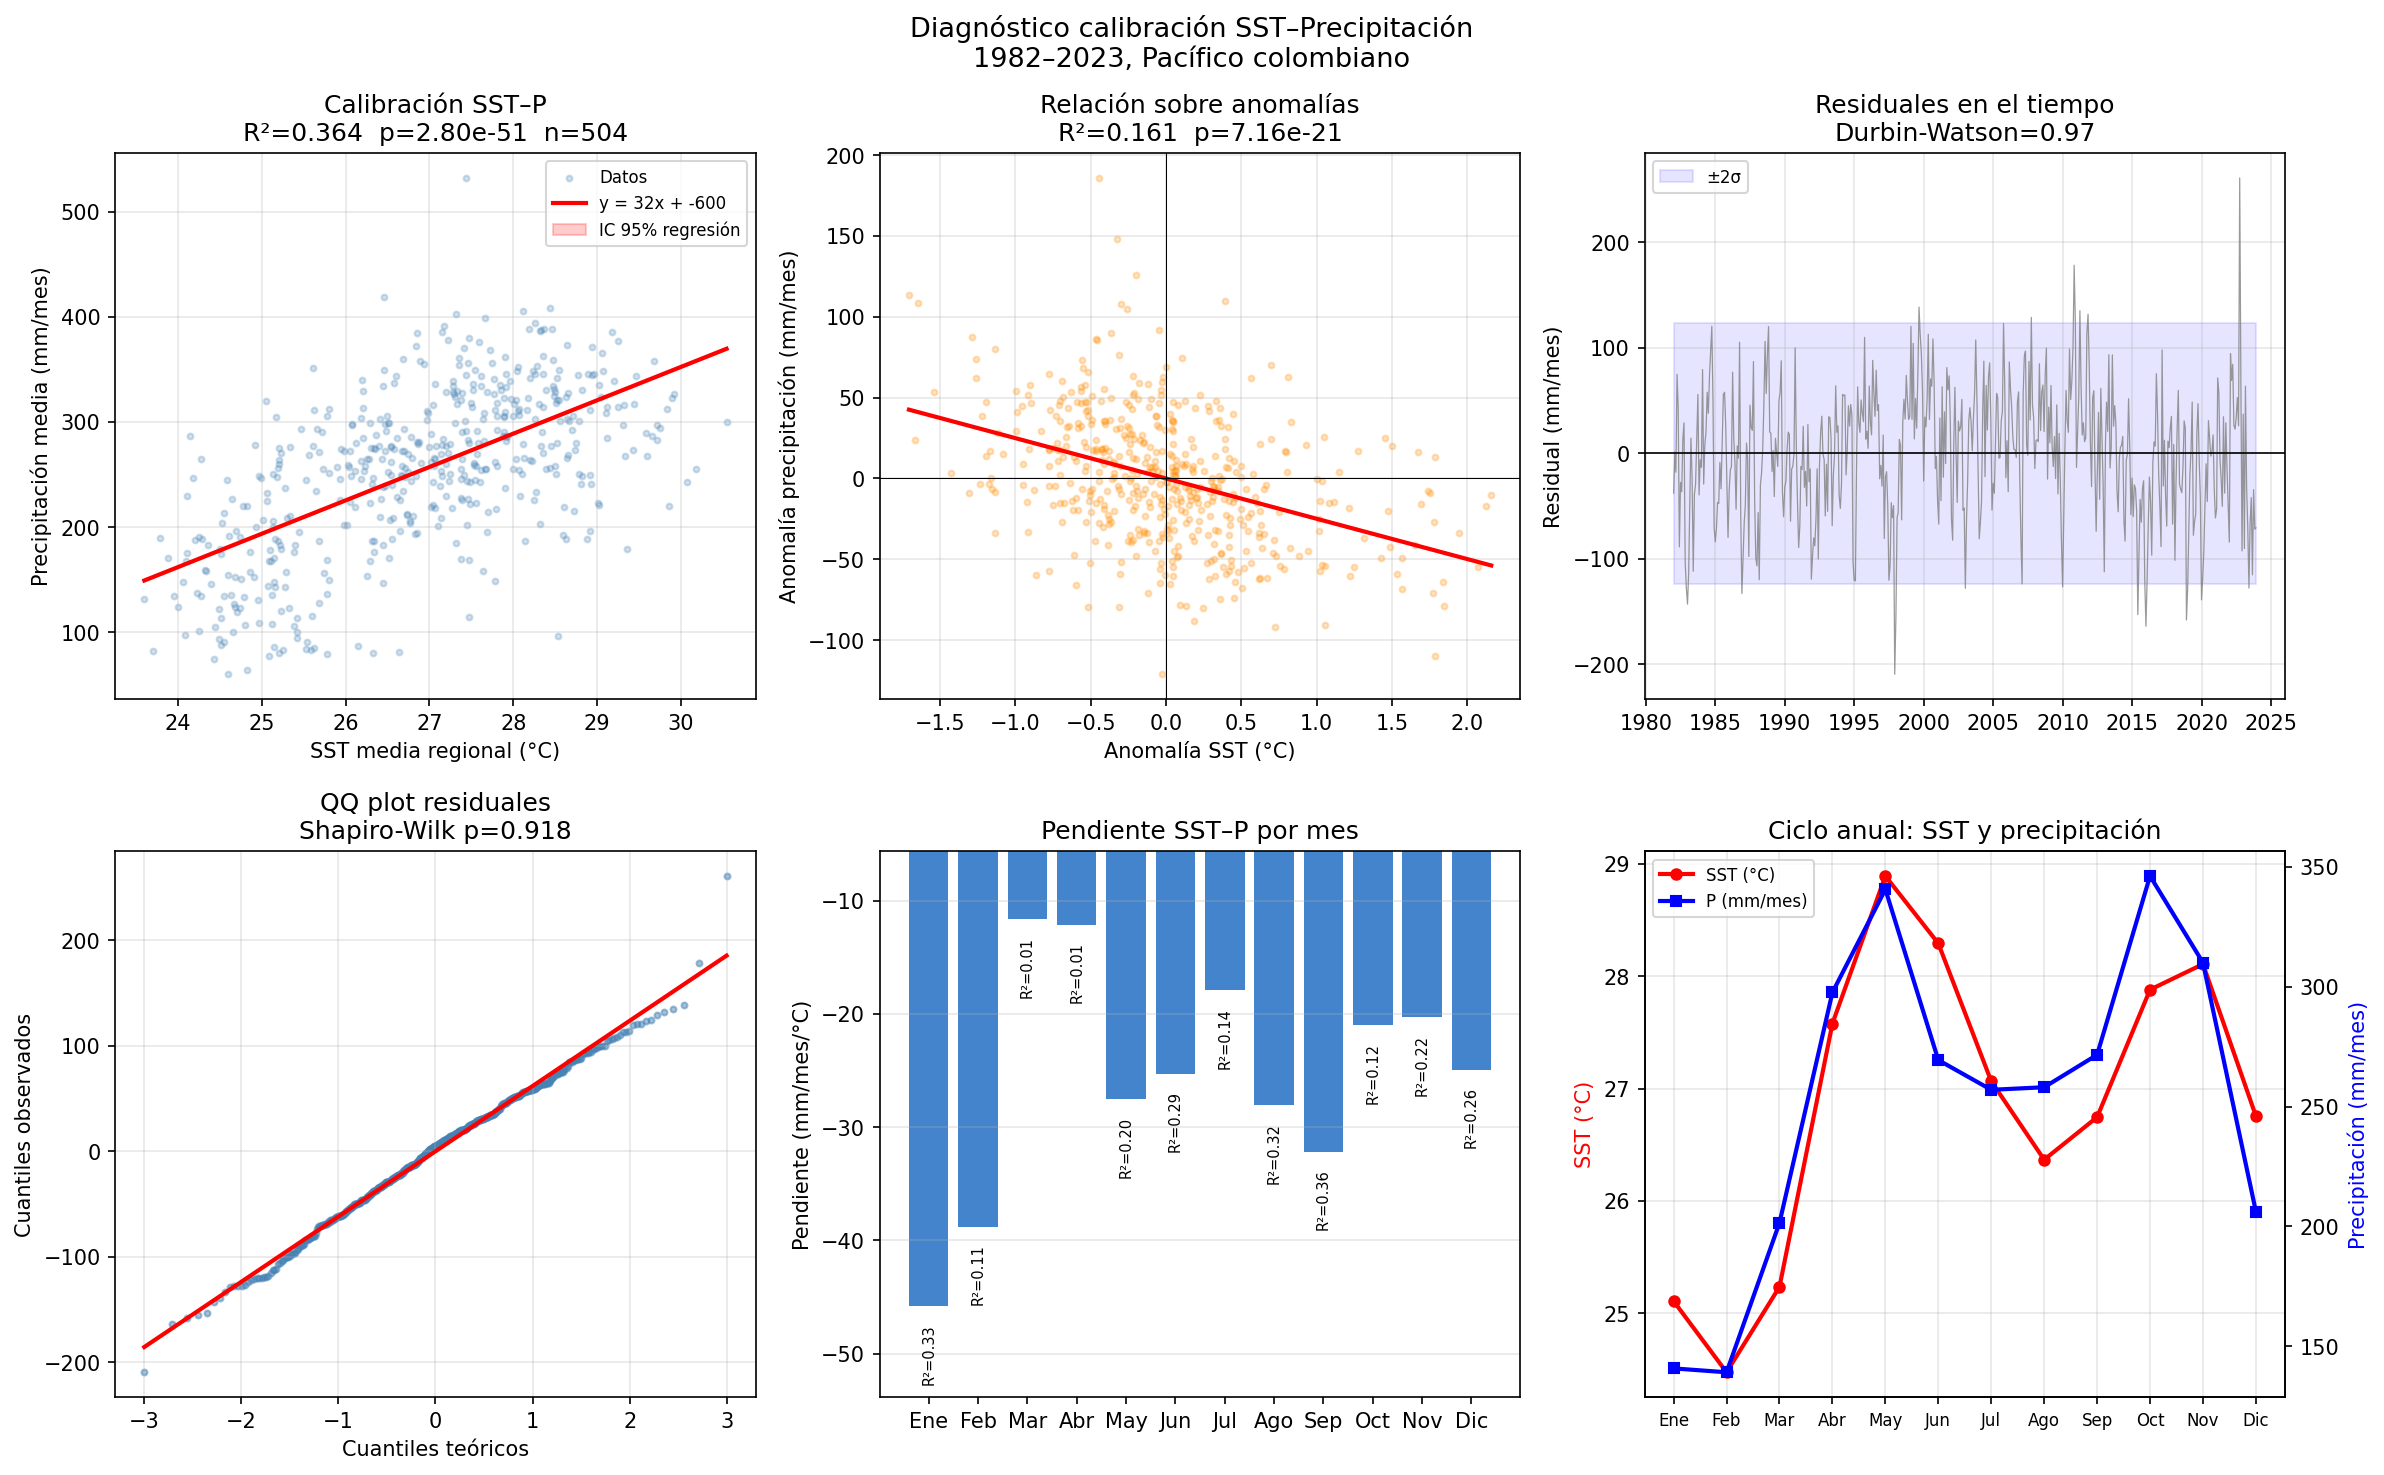
\includegraphics[width=\textwidth]{../fig_diagnostico_calibracion_sst_p.png}
	\caption{Diagn\'ostico de la calibraci\'on SST--precipitaci\'on (1982--2023). 
		(a)~Dispersi\'on SST media regional vs.\ precipitaci\'on media mensual 
		(CHIRPS) con recta de regresi\'on e IC 95\,\%. (b)~Misma relaci\'on sobre 
		anomal\'ias con ciclo estacional removido; la pendiente negativa indica que 
		la relaci\'on positiva en series brutas es de origen estacional. 
		(c)~Residuales de la regresi\'on en el tiempo; la banda azul indica $\pm 2\sigma$. 
		(d)~Gr\'afico QQ de los residuales; el Shapiro-Wilk ($p = 0.918$) confirma 
		normalidad. (e)~Pendiente SST--P por mes; todas las pendientes son negativas, 
		consistente con el resultado del panel (b). (f)~Ciclo anual de SST y 
		precipitaci\'on; la covariaci\'on estacional positiva explica la pendiente 
		global positiva del panel (a).}
	\label{fig:diagnostico_calibracion}
\end{figure}

Sin embargo, al remover el ciclo estacional la pendiente se invierte a 
$-24.9\,\text{mm\,mes}^{-1}\,^{\circ}\text{C}^{-1}$ ($R^2 = 0.161$), revelando que 
la relaci\'on positiva en series brutas no refleja causalidad SST$\rightarrow$P 
interanual sino la covariaci\'on estacional compartida: cuando la SST es alta 
(mayo--octubre), la precipitaci\'on tambi\'en lo es, pero ambas responden al mismo 
ciclo estacional y no existe una relaci\'on de causa a efecto directa entre ellas a 
escala interanual.

Este resultado se confirma al analizar la pendiente mes a mes, que resulta negativa en 
11 de los 12 meses, con los mayores valores absolutos entre agosto y octubre 
($R^2$ entre 0.26 y 0.36), precisamente cuando la variabilidad interanual asociada a 
ENSO es m\'as activa en el Pac\'ifico colombiano \cite{Ceron2021}. La \'unica pendiente 
positiva, en abril, tiene $R^2 \approx 0$ y no es estad\'isticamente significativa.

En cuanto a la calidad del ajuste, los residuales siguen una distribuci\'on 
aproximadamente normal (Shapiro-Wilk $p = 0.918$), lo que valida el uso del bootstrap 
para cuantificar la incertidumbre en la pendiente. No obstante, el estad\'istico de 
Durbin-Watson de 0.97 evidencia autocorrelaci\'on positiva en los residuales, lo que 
viola el supuesto de independencia de la regresi\'on lineal ordinaria y sugiere que los 
errores est\'andar reportados subestiman la incertidumbre real. Por estas razones, los 
cambios de precipitaci\'on estimados en la secci\'on siguiente deben interpretarse como 
cotas superiores de orden de magnitud, no como proyecciones cuantitativas.

\subsection{Cambio estimado en precipitaci\'on}

La Tabla~3 resume los cambios de precipitaci\'on estimados para cada escenario a partir 
de la pendiente calibrada y su intervalo de confianza bootstrap del 95\,\%.

\begin{table}[h]
	\centering
	\caption{Cambio estimado en precipitaci\'on por escenario. La precipitaci\'on 
		de referencia es 253.2\,mm\,mes$^{-1}$ (media 1982--2023). El IC 95\,\% se 
		obtuvo mediante bootstrap con 1\,000 remuestras.}
	\label{tab:delta_p}
	\begin{tabular}{lcccc}
		\hline
		Escenario & $\Delta$SST ($^{\circ}$C) & $\Delta$P (mm\,mes$^{-1}$) & 
		IC 95\,\% (mm\,mes$^{-1}$) & Cambio (\%) \\
		\hline
		SSP1-2.6 ($+1.5^{\circ}$C) & $+0.32$ & $+10.0$ & $[+8.9,\,+11.2]$  & $+4.0$ \\
		SSP2-4.5 ($+2.0^{\circ}$C) & $+0.42$ & $+13.3$ & $[+11.9,\,+14.9]$ & $+5.3$ \\
		SSP5-8.5 ($+4.0^{\circ}$C) & $+0.83$ & $+26.5$ & $[+23.5,\,+29.6]$ & $+10.4$ \\
		\hline
	\end{tabular}
\end{table}

La Figura~11 ilustra estos resultados con sus barras de error. Los tres escenarios 
predicen un incremento en la precipitaci\'on de la regi\'on costera y andina adyacente, 
con una respuesta aproximadamente lineal al forzamiento t\'ermico. Dada la advertencia 
sobre el origen estacional de la relaci\'on SST--P, estos valores no deben interpretarse 
como proyecciones cuantitativas sino como una estimaci\'on de orden de magnitud del 
impacto hidrol\'ogico potencial bajo cada escenario.

\begin{figure}[h]
	\centering
	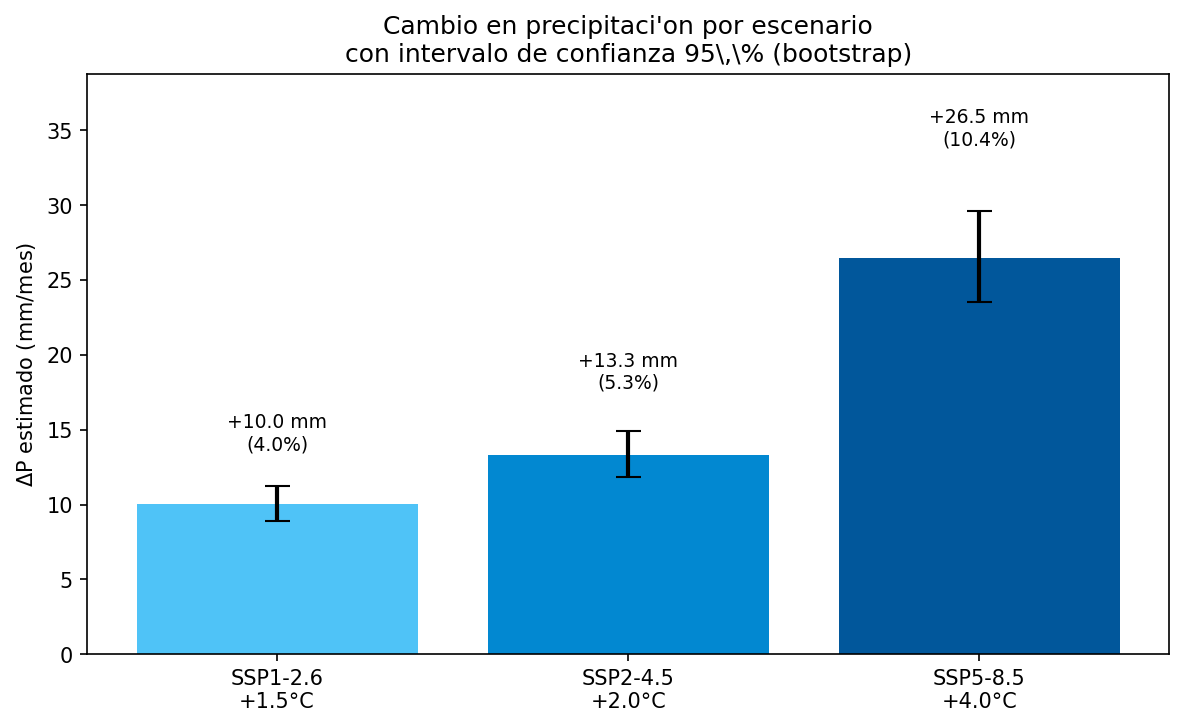
\includegraphics[width=0.75\textwidth]{../fig_incertidumbre_delta_p.png}
	\caption{Cambio estimado en precipitaci\'on mensual ($\Delta$P) sobre la 
		regi\'on costera y andina adyacente (2--8$^{\circ}$N, 73--78$^{\circ}$W) 
		para los tres escenarios de calentamiento atmosf\'erico. Las barras de error 
		indican el intervalo de confianza del 95\,\% obtenido mediante bootstrap con 
		1\,000 remuestras sobre la pendiente de la relaci\'on SST--precipitaci\'on. 
		La precipitaci\'on de referencia es 253.2\,mm\,mes$^{-1}$ (media 1982--2023).}
	\label{fig:delta_p_escenarios}
\end{figure}

\end{document}
